Let the sales of the product x,y and z per market be denoted by  matrix A
\begin{align}
\begin{blockarray}{cccc}
\text{x} & \text{y} & \text{z} \\
\begin{block}{(ccc)(c)}
10000 & 2000 & 18000 & \text{Market-I}\\
6000 & 20000 & 8000 & \text{Market-II} \\
\end{block}
\end{blockarray}
\end{align}
\begin {enumerate}
\item
Let the unit sale price of the products x,y and z per market be denoted by matrix B
\begin{align}
\vec{B}=\myvec{2.50\\1.50\\1.00}
\end{align}
Total Revenue in Market-I and Market-II
\begin{align}
\vec{A}\vec{B}&=\myvec{10000&2000&18000\\6000&20000&8000}\myvec{2.50\\1.50\\1.00}\\
&=\myvec{46000\\53000}
\end{align}
\item
Let the unit cost price of the products x,y and z per market be denoted by matrix C
\begin{align}
\vec{C}=\myvec{2.00\\1.00\\0.50}
\end{align}
Total cost of Market-I and Market-II
\begin{align}
\vec{A}\vec{C}&=\myvec{10000&2000&18000\\6000&20000&8000}\myvec{2.00\\1.00\\0.50}\\
&=\myvec{31000\\36000}
\end{align}
$\therefore$ Gross Profit = Total revenue - Total cost
\begin{align}
\vec{A}\vec{B}-\vec{A}\vec{C}&=\myvec{46000\\53000} - \myvec{31000\\36000}  \\
&=\myvec{15000\\17000}
\end{align}
$\therefore$ Total profit in Market-I = 15000
Total profit in Market-II =17000
\end{enumerate}
%
\begin{figure}[!ht]
\centering
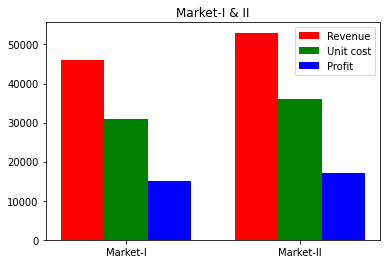
\includegraphics[width=\columnwidth]{solutions/su2021/45/FIGURE.png}
\caption{Revenue,Sales \& Profit Of Market-I \& II}
\label{matrix/2/45/fig:Profit}	
\end{figure}